\chapter{Background Study}
\label{chap2}
%##########################################


\vspace*{45 ex}
%##########################################



\paragraph*{Outline:} This chapter presents the following:
\begin{enumerate}
\setlength{\itemsep}{-0.3em}
\item Introduction
\item Machine Learning
\item Neural Networks
\item Computer Vision
\item Convolutional neural networks
\end{enumerate}

%+++++++++++++++++++++++++++++++++++++++++++++++++++++++++++++++++
\newpage

\section{Introduction}
In this chapter, we provide the theoretical background necessary for understanding the methods discussed in the next chapter. First, we discuss relevant details of machine learning, neural networks, and computer vision. Finally, we explain how these disciplines are combined in convolutional neural networks.

\section{Machine Learning}
Learning algorithms are widely used in computer vision applications. Before considering image related tasks, we are going to have a brief look at basics of machine learning.

Machine learning has emerged as a useful tool for modeling problems that are otherwise difficult to formulate exactly. Classical computer programs are explicitly programmed by hand to perform a task. With machine learning, some portion of the human contribution is replaced by a learning algorithm. As availability of computational capacity and data has increased, machine learning has become more and more practical over the years, to the point of being almost ubiquitous.

\subsection{Types}
A typical way of using machine learning is supervised learning. A learning algorithm is shown multiple examples that have been annotated or labeled by humans. For example, in the object detection problem we use training images where humans have marked the locations and classes of relevant objects. After learning from the examples, the algorithm is able to predict the annotations or labels of previously unseen data. Classification and regression are the most important task types. In classification, the algorithm attempts to predict the correct class of a new piece of data based on the training data. In regression, instead of discrete classes, the algorithm tries to predict a continuous output.

In unsupervised learning, the algorithm attempts to learn useful properties of the data without a human teacher telling what the correct output should be. Classical example of unsupervised learning is clustering. More recently, especially with the advent of deep learning technologies, unsupervised preprocessing has become a popular tool in supervised learning tasks for discovering useful representations of the data.

\subsection{Features}
Some kind of preprocessing is almost always needed. Preprocessing the data into a new, simpler variable space is called feature extraction. Often, it is impractical or impossible to use the full-dimensional training data directly. Rather, detectors are programmed to extract interesting features from the data, and these features are used as input to the machine learning algorithm.

In the past, the feature detectors were often hand-crafted. The problem with this approach is that we do not always know in advance, which features are interesting. The trend in machine learning has been towards learning the feature detectors as well, which enables using the complete data.

\subsection{Generalization}
Since the training data cannot include every possible instance of the inputs, the learning algorithm has to be able to generalize in order to handle unseen data points. Too simple model estimate can fail to capture important aspects of the true model. On the other hand, too complex methods can overfit by modeling unimportant details and noise, which also leads to bad generalization. Typically, overfitting happens when a complex method is used in conjunction with too little training data. An overfitted model learns to model the known examples but does not understand what connects them.

The performance of the algorithm can be evaluated from the quality and quantity of errors. A loss function, such as mean squared error, is used to assign a cost to the errors. The objective in the training phase is to minimize this loss.

\section{Neural Networks}
Neural networks are a popular type of machine learning model. A special case of a neural network called the convolutional neural network (CNN) is the primary focus of this thesis. Before discussing CNNs, we will discuss how regular neural networks work.

\subsection{Origins}
Neural networks were originally called artificial neural networks, because they were developed to mimic the neural function of the human brain. Pioneering research includes the threshold logic unit by Warren McCulloch and Walter Pitts in 1943 and the perceptron by Frank Rosenblatt in 1957. Even though the inspiration from biology is apparent, it would be misleading to overemphasize the connection between artificial neurons and biological neurons or neuroscience. The human brain contains approximately 100 billion neurons operating in parallel. Artificial neurons are mathematical functions implemented on more-or-less serial computers. Research into neural networks is mostly guided by developments in engineering and mathematics rather than biology.

\begin{figure}
	\centering
	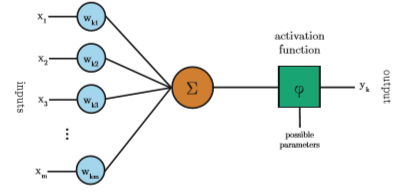
\includegraphics[width=0.7\linewidth]{img1}
	\caption{An artificial neuron.} \href{https://www.semanticscholar.org/paper/Object-detection-from-images-using-convolutional-Stenroos/a6ee78ea9c68d99d6545227fed925a721337bb16/figure/0}{link}
	\label{fig:img1}
\end{figure}


An artificial neuron based on the McCulloch-Pitts model is shown in Figure 2.1. The neuron k receives m input parameters $x_{j}$. The neuron also has m weight parameters $w_{kj}$. The weight parameters often include a bias term that has a matching dummy input with a fixed value of 1. The inputs and weights are linearly combined and summed. The sum is then fed to an activation function $\phi$ that produces the output $y_{k}$ of the neuron:\[y_{k} = \phi(s_{k}) = \phi( \sum_{j=0}^{m}w_{kj}x_{j}) \]

The neuron is trained by carefully selecting the weights to produce a desired output for each input.


\subsection{Multi-layer networks}
A neural network is a combination of artificial neurons. The neurons are typically grouped into layers. In a fully-connected feed-forward multi-layer network, shown in Figure 2.2, each output of a layer of neurons is fed as input to each neuron of the next layer. Thus, some layers process the original input data, while some process data received from other neurons. Each neuron has a number of weights equal to the number of neurons in the previous layer.
\begin{figure}
	\centering
	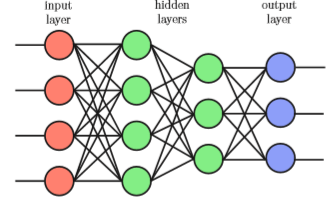
\includegraphics[width=0.7\linewidth]{img2}
	\caption{A fully-connected multi-layer neural network.} \href{https://www.semanticscholar.org/paper/Object-detection-from-images-using-convolutional-Stenroos/a6ee78ea9c68d99d6545227fed925a721337bb16/figure/1}{link}
	\label{fig:img2}
\end{figure}

A multi-layer network typically includes three types of layers: an input layer, one or more hidden layers and an output layer. The input layer usually merely passes data along without modifying it. Most of the computation happens in the hidden layers. The output layer converts the hidden layer activations to an output, such as a classification. A multilayer feed-forward network with at least one hidden layer can function as a universal approximator i.e. can be constructed to compute almost any function.

In this thesis, we will mostly discuss fully-connected networks and convolutional networks (see section 2.5). Convolutional networks utilize parameter sharing and have limited connections compared to fully-connected networks. Other network types, such as recurrent networks, are outside the scope of this thesis.

\subsection{Back-propagation}
A neural network is trained by selecting the weights of all neurons so that the network learns to approximate target outputs from known inputs. It is difficult to solve the neuron weights of a multi-layer network analytically. The back-propagation algorithm provides a simple and effective solution to solving the weights iteratively. The classical version uses gradient descent as optimization method. Gradient descent can be quite time-consuming and is not guaranteed to find the global minimum of error, but with proper configuration (known in machine learning as hyperparameters) works well enough in practice. 

In the first phase of the algorithm, an input vector is propagated forward through the neural network. Before this, the weights of the network neurons have been initialized to some values, for example small random values. The received output of the network is compared to the desired output (which should be known for the training examples) using a loss function. The gradient of the loss function is then computed. This gradient is also called the error value. When using mean squared error as the loss function, the output layer error value is simply the difference between the current and desired output. 

The error values are then propagated back through the network to calculate the error values of the hidden layer neurons. The hidden neuron loss function gradients can be solved using the chain rule of derivatives. Finally, the neuron weights are updated by calculating the gradient of the weights and subtracting a proportion of the gradient from the weights. This ratio is called the learning rate. The learning rate can be fixed or dynamic. After the weights have been updated, the algorithm continues by executing the phases again with different input until the weights converge. In the above description, we have described online learning that calculates the weight updates after each new input. Online learning can lead to “zig-zagging” behaviour, where the single data point estimate of the gradient keeps changing direction and does not approach the minimum directly. Another way of computing the updates is full batch learning, where we compute the weight updates for the complete dataset. This is quite computationally heavy and has other drawbacks. A compromise version is mini-batch learning, where we use only some portion of the training set for each update. Mathematical descriptions of the algorithm are readily available in other works.

\subsection{Deep learning}

Modern neural networks are often called deep neural networks. Even though multi-layer neural networks have existed since the 1980s, several reasons prevented the effective training of networks with multiple hidden layers.

One of the main problems is the curse of dimensionality. As the number of variables increases, the number of different configurations of the variables grows exponentially. As the number of configurations increases, the number of training samples should increase in equal measure. Collecting a training dataset of sufficient size is time-consuming and costly or outright impossible. 

Fortunately, real-world data is not uniformly distributed and often involves a structure, where the interesting information lies on a low-dimensional manifold. The manifold hypothesis assumes that most data configurations are invalid or rare. We can decrease dimensionality by learning to represent the data using the coordinates of the manifold. Another way to improve generalization is to assume local constancy. This means assuming that the function that the neural network learns to approximate should not change much within a small region.

In the past ten years, neural networks have had a renaissance, mainly because of the availability of more powerful computers and larger datasets. In early 2000s, it was discovered that neural networks could be trained efficiently using graphics processing units. GPUs are more efficient for the task than traditional CPUs and provide a relatively cheap alternative to specialist hardware. Today, researchers typically use high-end consumer graphic cards, such as NVIDIA Tesla K40.

Other more theoretical breakthroughs include replacing mean-squared error functions with cross-entropy based functions and replacing sigmoidal activation functions with rectified linear units.

With deep learning, there is less need for hand-tuned machine learning solutions that were used previously. A classical pattern detection system, for example, includes a hand-tuned feature detection phase before a machine learning phase. The deep learning equivalent consists of a single neural network. The lower layers of the neural network learn to recognize the basic features, which are then fed forward to higher layers of the network.

\subsection{Activation function type}

The activation function  determines the final output of each neuron. It is important to select the function properly in order to create an effective network. 


Early researchers found that perceptrons and other linear systems had severe drawbacks, being unable to solve problems that were not linearly separable, such as the XOR-problem. Sometimes, linear systems can solve these kinds of problems using hand-crafted feature detectors, but this is not the most advantageous use of machine learning. Simply adding layers does not help either, because a network composed of linear neurons remains linear no matter how many layers it has.

A light-weight and effective way of creating a non-linear network is using rectified linear units (ReLu). A rectified linear function generates the output using a ramp function such as:\[\phi(s) = max(0,s)\].

This type of function is easy to compute and differentiate (for backpropagation). The function is not differentiable at zero, but this has not prevented its use in practice. ReLus have become quite popular lately, often replacing sigmoidal activation functions, which have smooth derivatives but suffer from gradient saturation problems and slower computation. For multi-class classification problems, the softmax activation function is used in the output layer of the network:\[\phi(s) = \frac{exp(s_{k})}{\sum_{k=1}^{K}exp(s_{k})}\].

The softmax function takes a vector of K arbitrarily large values and outputs a vector of K values that range between 0...1 and sum to 1. The values output by the softmax unit can be utilized as class probabilities.


\section{Computer vision}
Next, we are going to discuss computer vision in general and explore the primary subject of this thesis, object detection, as a subproblem of computer vision.

\subsection{Overview}
Computer vision deals with the extraction of meaningful information from the contents of digital images or video. This is distinct from mere image processing, which involves manipulating visual information on the pixel level. Applications of computer vision include image classification, visual detection, 3D scene reconstruction from 2D images, image retrieval, augmented reality, machine vision and traffic automation.

Today, machine learning is a necessary component of many computer vision algorithms. Such algorithms can be described as a combination of image processing and machine learning. Effective solutions require algorithms that can cope with the vast amount of information contained in visual images, and critically for many applications, can carry out the computation in real time.

\subsection{Object detection}
Object detection is one of the classical problems of computer vision and is often described as a difficult task. In many respects, it is similar to other computer vision tasks, because it involves creating a solution that is invariant to deformation and changes in lighting and viewpoint. What makes object detection a distinct problem is that it involves both locating and classifying regions of an image. The locating part is not needed in, for example, whole image classification.

To detect an object, we need to have some idea where the object might be and how the image is segmented. This creates a type of chicken-and-egg problem, where, to recognize the shape (and class) of an object, we need to know its location, and to recognize the location of an object, we need to know its shape. Some visually dissimilar features, such as the clothes and face of a human being, may be parts of the same object, but it is difficult to know this without recognizing the object first. On the other hand, some objects stand out only slightly from the background, requiring separation before recognition.

Low-level visual features of an image, such as a saliency map, may be used as a guide for locating candidate objects. The location and size is typically defined using a bounding box, which is stored in the form of corner coordinates. Using a rectangle is simpler than using an arbitrarily shaped polygon, and many operations, such as convolution, are performed on rectangles in any case. The sub-image contained in the bounding box is then classified by an algorithm that has been trained using machine learning. The boundaries of the object can be further refined iteratively, after making an initial guess.

During the 2000s, popular solutions for object detection utilized feature descriptors, such as scale-invariant feature transform (SIFT) developed by David Lowe in 1999 and histogram of oriented gradients (HOG) popularized in 2005. In the 2010s, there has been a shift towards utilizing convolutional neural networks.

Before the widescale adoption of CNNs, there were two competing solutions for generating bounding boxes. In the first solution, a dense set of region proposals is generated and then most of these are rejected. This typically involves a sliding window detector. In the second solution, a sparse set of bounding boxes is generated using a region proposal method, such as Selective Search. Combining sparse region proposals with convolutional neural networks has provided good results and is currently popular.

\section{Convolutional neural networks}
Next, we are going to discuss why and how convolutional neural networks (CNN) are used and describe their history.

\subsection{Justification}
The problem with solving computer vision problems using traditional neural networks is that even a modestly sized image contains an enormous amount of information (see section 2.2.4 on deep learning and the curse of dimensionality).

A monochrome 620x480 image contains 297 600 pixels. If each pixel intensity of this image is input separately to a fully-connected network, each neuron requires 297 600 weights. A 1920x1080 full HD image would require 2,073,600 weights. If the images are polychrome, the amount of weights is multiplied by the amount of colour channels (typically three). Thus, we can see that the overall number of free parameters in the network quickly becomes extremely large as the image size increases. Too large models cause overfitting and slow performance.

Furthermore, many pattern detection tasks require that the solution is translation invariant. It is inefficient to train neurons to separately recognize the same pattern in the left-top corner and in the right-bottom corner of an image. A fully-connected neural network fails to take this kind of structure into account. 

\subsection{Basic structure}
The basic idea of the CNN was inspired by a concept in biology called the receptive field. Receptive fields are a feature of the animal visual cortex. They act as detectors that are sensitive to certain types of stimulus, for example, edges. They are found across the visual field and overlap each other.

This biological function can be approximated in computers using the convolution operation. In image processing, images can be filtered using convolution to produce different visible effects. Figure 2.3 shows how a hand-selected convolutional filter detects horizontal edges from an image, functioning similarly to a receptive field.

The discrete convolution operation between an image f and a filter matrix g is defined as:\[h[x,y] = f[x,y]*g[x,y] = \sum_{n}\sum_{m}f[n,m]g[x-n,y-m]\].

In effect, the dot product of the filter g and a sub-image of f (with same dimensions as g) centred on coordinates x,y produces the pixel value of h at coordinates x,y. The size of the receptive field is adjusted by the size of the filter matrix. Aligning the filter successively with every sub-image of f produces the of output pixel matrix h. In the case of neural networks, the output matrix is also called an feature map (or an activation map after computing the activation function). Edges need to be treated as a special case. If image f is not padded, the output size decreases slightly with every convolution.

A set of convolutional filters can be combined to form a convolutional layer of a neural network. The matrix values of the filters are treated as neuron parameters and trained using machine learning. The convolution operation replaces the multiplication operation of a regular neural network layer. Output of the layer is usually described as a volume. The height and width of the volume depend on the dimensions of the activation map. The depth of the volume depends on the number of filters.

\begin{figure}
	\centering
	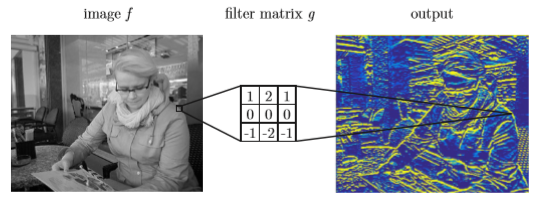
\includegraphics[width=0.7\linewidth]{img3}
	\caption{ Detecting horizontal edges from an image using convolution filtering.} \href{https://www.semanticscholar.org/paper/Object-detection-from-images-using-convolutional-Stenroos/a6ee78ea9c68d99d6545227fed925a721337bb16/figure/2}{link}
	\label{fig:img3}
\end{figure}

Since the same filters are used for all parts of the image, the number of free parameters is reduced drastically compared to a fully-connected neural layer. The neurons of the convolutional layer mostly share the same parameters and are only connected to a local region of the input. Parameter sharing resulting from convolution ensures translation invariance. An alternative way of describing the convolutional layer is to imagine a fully-connected layer with an infinitely strong prior placed on its weights. This prior forces the neurons to share weights at different spatial locations and to have zero weight outside the receptive field.

\begin{figure}
	\centering
	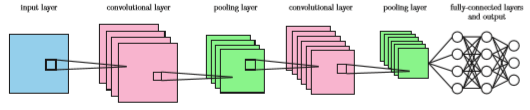
\includegraphics[width=0.7\linewidth]{img4}
	\caption{ An example of a convolutional network.} \href{https://www.semanticscholar.org/paper/Object-detection-from-images-using-convolutional-Stenroos/a6ee78ea9c68d99d6545227fed925a721337bb16/figure/3}{link}
	\label{fig:img4}
\end{figure}

Successive convolutional layers (often combined with other types of layers, such as pooling described below) form a convolutional neural network (CNN). An example of a convolutional network is shown in figure 2.4. The backpropagation training algorithm, described in section 2.2.3, is also applicable to convolutional networks. In theory, the layers closer to the input should learn to recognize low-level features of the image, such as edges and corners, and the layers closer to the output should learn to combine these features to recognize more meaningful shapes. In this thesis, we are interested in studying whether convolutional networks can learn to recognize complete objects.


\subsection{ Pooling and stride}
To make the network more manageable for classification, it is useful to decrease the activation map size in the deep end of the network. Generally,the deep layers of the network require less information about exact spatial locations of features, but require more filter matrixes to recognize multiple high-level patterns. By reducing the height and width of the data volume, we can increase the depth of the data volume and keep the computation time at a reasonable level. 

There are two ways of reducing the data volume size. One way is to include a pooling layer after a convolutional layer. The layer effectively down-samples the activation maps. Pooling has the added effect of making the resulting network more translation invariant by forcing the detectors to be less precise. However, pooling can destroy information about spatial relationships between subparts of patterns. Typical pooling method is max-pooling. Max-pooling simply outputs the maximum value within a rectangular neighbourhood of the activation map.

Another way of reducing the data volume size is adjusting the stride parameter of the convolution operation. The stride parameter controls whether the convolution output is calculated for a neighbourhood centred on every pixel of the input image (stride 1) or for every nth pixel (stride n). Research has shown that pooling layers can often be discarded without loss in accuracy by using convolutional layers with larger stride value. The stride operation is equivalent to using a fixed grid for pooling.

\subsection{Additional layers}
The convolutional layer typically includes a non-linear activation function, such as a rectified linear activation function (see subsection 2.2.5). Activations are sometimes described as a separate layer between the convolutional layer and the pooling layer.

Some systems, such as, also implement a layer called local response normalization, which is used as a regularization technique. Local response normalization mimics a function of biological neurons called lateral inhibition, which causes excited neurons to decrease the activity of neighbouring neurons. However, other regularization techniques are currently more popular and these are discussed in the next section.

The final hidden layers of a CNN are typically fully-connected layers. A fully-connected layer can capture some interesting relationships parameter-sharing convolutional layers cannot. However, a fully connected layer requires a sufficiently small data volume size in order to be practical. Pooling and stride settings can be used to reduce the size of the data volume that reaches the fully-connected layers. A convolutional network that does not include any fully-connected layers, is called a fully convolutional network (FCN).

If the network is used for classification, it usually includes a softmax output layer (see also section 2.2.5). The activations of the topmost layers can also be used directly to generate a feature representation of an image. This means that the convolutional network is used as a large feature detector.

\subsection{Regularization and data augmentation}
Regularization refers to methods that are used to reduce overfitting by introducing additional constraints or information to the machine learning system. A classical way of using regularization in neural networks is adding a penalty term to the objective/loss function that penalizes certain types of weights. The parameter sharing feature of convolutional networks is another example of regularization.

There are several regularization techniques that are specific to deep neural networks. A popular technique called dropout attempts to reduce the co-adaptation of neurons. This is achieved by randomly dropping out neurons during training, meaning that a slightly different neural network is used for each training sample or minibatch. This causes the system not to depend too much on any single neuron or connection and provides an effective yet computationally inexpensive way of implementing regularization. In convolutional networks, dropout is typically used in the final fully-connected layers.

Overfitting can also be reduced by increasing the amount of training data. When it is not possible to acquire more actual samples, data augmentation is used to generate more samples from the existing data. For classification using convolutional networks, this can be achieved by computing transformations of the input images that do not alter the perceived object classes, yet provide additional challenge to the system. The images can be, for example, flipped, rotated or subsampled with different crops and scales. Also, noise can be added to the input images.

\subsection{Development}
Convolutional neural networks were one of the first successful deep neural networks. The Neocognitron, developed by Fukushima in 1980s, provided a neural network model for translation-invariant object recognition, inspired by biology. Le Cun et al. combined this method with a learning algorithm, i.e. back-propagation. These early solutions were mostly used for handwritten character recognition.

After providing some promising results, the neural network methods faded in prominence and were mostly replaced by support vector machines. Then, in 2012, Krizhevsky et al. achieved excellent results on the ImageNet Large Scale Visual Recognition Challenge (ILSVRC) dataset by combining Le Cun’s method with recent fine-tuning methods for deep learning. These results popularised CNNs and led to the development of new powerful object detection methods described in chapter 3.

For the 2014 ImageNet challenge, Simonyan and Zisserman explored the effect of increasing the depth of a convolutional network on localisation and classification accuracy. The team achieved results that improved the then state-of-the-art by using convolutional networks 16 and 19 layers deep. The 16-layer architecture includes 13 convolutional layers (with 3x3 filters), 5 pooling layers (2x2 neighbourhood max-pooling) and 3 fully-connected layers. All hidden layers use rectified (ReLu) activations. The fully-connected layers reduce 4096 channels down to 1000 softmax outputs and are regularized using dropout. This form of network is referred to as VGG-16 later in this thesis.

The current (2016) winner of the object detection category in the ImageNet challenge is also CNN-based. The method uses a combination of CRAFT region proposal generation, gated bi-directional CNN, clustering, landmark generation and ensembling.

 
%\max_{{P^{\circ}_t(j)}}
%\section{Summary}
%In this chapter, we describe .......    
